\documentclass[journal]{vgtc}                % final (journal style)
%\documentclass[review,journal]{vgtc}         % review (journal style)
%\documentclass[widereview]{vgtc}             % wide-spaced review
%\documentclass[preprint,journal]{vgtc}       % preprint (journal style)

%% Uncomment one of the lines above depending on where your paper is
%% in the conference process. ``review'' and ``widereview'' are for review
%% submission, ``preprint'' is for pre-publication, and the final version
%% doesn't use a specific qualifier.

%% Please use one of the ``review'' options in combination with the
%% assigned online id (see below) ONLY if your paper uses a double blind
%% review process. Some conferences, like IEEE Vis and InfoVis, have NOT
%% in the past.

%% Please note that the use of figures other than the optional teaser is not permitted on the first page
%% of the journal version.  Figures should begin on the second page and be
%% in CMYK or Grey scale format, otherwise, colour shifting may occur
%% during the printing process.  Papers submitted with figures other than the optional teaser on the
%% first page will be refused. Also, the teaser figure should only have the
%% width of the abstract as the template enforces it.

%% These few lines make a distinction between latex and pdflatex calls and they
%% bring in essential packages for graphics and font handling.
%% Note that due to the \DeclareGraphicsExtensions{} call it is no longer necessary
%% to provide the the path and extension of a graphics file:
%% 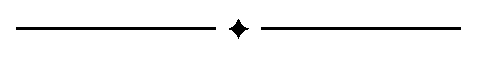
\includegraphics{diamondrule} is completely sufficient.
%%
\ifpdf%                                % if we use pdflatex
  \pdfoutput=1\relax                   % create PDFs from pdfLaTeX
  \pdfcompresslevel=9                  % PDF Compression
  \pdfoptionpdfminorversion=7          % create PDF 1.7
  \ExecuteOptions{pdftex}
  \usepackage{graphicx}                % allow us to embed graphics files
  \usepackage{hyperref}
  \hypersetup{
      colorlinks=true,
      linkcolor=blue,
      filecolor=magenta,      
      urlcolor=cyan,
  }
  \urlstyle{same}
  \DeclareGraphicsExtensions{.pdf,.png,.jpg,.jpeg} % for pdflatex we expect .pdf, .png, or .jpg files
\else%                                 % else we use pure latex
  \ExecuteOptions{dvips}
  \usepackage{graphicx}                % allow us to embed graphics files
  \DeclareGraphicsExtensions{.eps}     % for pure latex we expect eps files
\fi%

%% it is recomended to use ``\autoref{sec:bla}'' instead of ``Fig.~\ref{sec:bla}''
\graphicspath{{figures/}{pictures/}{images/}{./}} % where to search for the images

\usepackage{microtype}                 % use micro-typography (slightly more compact, better to read)
\PassOptionsToPackage{warn}{textcomp}  % to address font issues with \textrightarrow
\usepackage{textcomp}                  % use better special symbols
\usepackage{listings}
\raggedbottom
\usepackage{mathptmx}                  % use matching math font
\usepackage{times}                     % we use Times as the main font
\renewcommand*\ttdefault{txtt}         % a nicer typewriter font
\usepackage{cite}                      % needed to automatically sort the references
\usepackage{tabu}                      % only used for the table example
\usepackage{booktabs}                  % only used for the table example
%% We encourage the use of mathptmx for consistent usage of times font
%% throughout the proceedings. However, if you encounter conflicts
%% with other math-related packages, you may want to disable it.

%% In preprint mode you may define your own headline.
%\preprinttext{To appear in IEEE Transactions on Visualization and Computer Graphics.}

%% If you are submitting a paper to a conference for review with a double
%% blind reviewing process, please replace the value ``0'' below with your
%% OnlineID. Otherwise, you may safely leave it at ``0''.
\onlineid{0}

%% declare the category of your paper, only shown in review mode
\vgtccategory{Research}
%% please declare the paper type of your paper to help reviewers, only shown in review mode
%% choices:
%% * algorithm/technique
%% * application/design study
%% * evaluation
%% * system
%% * theory/model
\vgtcpapertype{please specify}

%% Paper title.
\title{Interactive Solar System Map Project}

%% This is how authors are specified in the journal style

%% indicate IEEE Member or Student Member in form indicated below
\author{Connor Sedwick, Tasnia Kabir}
%\authorfooter{
%% insert punctuation at end of each item

%}

%% Abstract section.
\abstract{Considering the lack of interactive solar system maps, we propose to design one that allows users to view data for individual celestial bodies by clicking on the visible bodies and reading the list of specific attributes and data for that body. %
} % end of abstract

%% Keywords that describe your work. Will show as 'Index Terms' in journal
%% please capitalize first letter and insert punctuation after last keyword
\keywords{}

%% ACM Computing Classification System (CCS). 
%% See <http://www.acm.org/class/1998/> for details.
%% The ``\CCScat'' command takes four arguments.

%\CCScatlist{ % not used in journal version
 %\CCScat{K.6.1}{Management of Computing and Information Systems}%
%{Project and People Management}{Life Cycle};
 %\CCScat{K.7.m}{The Computing Profession}{Miscellaneous}{Ethics}
%}

%% Uncomment below to include a teaser figure.
\teaser{
  \centering
  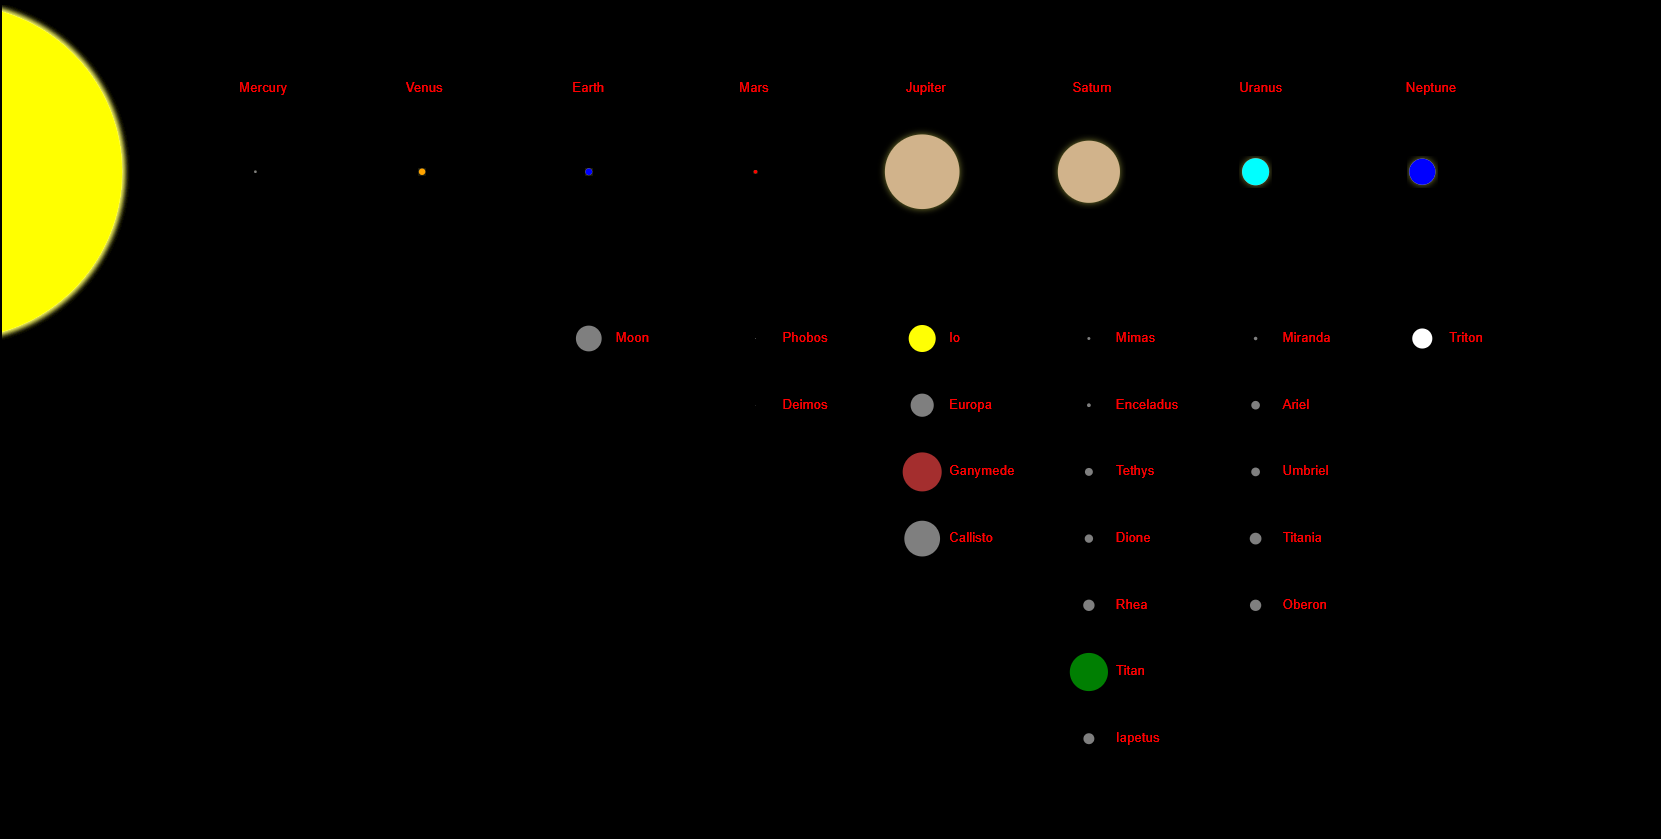
\includegraphics[width=\linewidth]{system-map}
  \caption{The current layout of our visualization.}
	\label{fig:teaser}
}

%% Uncomment below to disable the manuscript note
\renewcommand{\manuscriptnotetxt}{}

%% Copyright space is enabled by default as required by guidelines.
%% It is disabled by the 'review' option or via the following command:
%\nocopyrightspace

\vgtcinsertpkg

%%%%%%%%%%%%%%%%%%%%%%%%%%%%%%%%%%%%%%%%%%%%%%%%%%%%%%%%%%%%%%%%
%%%%%%%%%%%%%%%%%%%%%% START OF THE PAPER %%%%%%%%%%%%%%%%%%%%%%
%%%%%%%%%%%%%%%%%%%%%%%%%%%%%%%%%%%%%%%%%%%%%%%%%%%%%%%%%%%%%%%%%

\begin{document}

%% The ``\maketitle'' command must be the first command after the
%% ``\begin{document}'' command. It prepares and prints the title block.

%% the only exception to this rule is the \firstsection command
%%%%%%%%%%%%%%%%%%%%%%%%%%%%%%%%%%%%%%%%%%%%%%%%%%%%%%%%%%%%%%%%%%%%
\maketitle
\section{Introduction}
%% \section{Introduction} %for journal use above \firstsection{..} instead
Currently, there are not many interactive ways to learn about the celestial bodies in our solar system. Though there are many diagrams and images available online showing the location and orbits of celestial bodies, they fail to provide detailed information on the properties of celestial bodies: mass, density, gravity, satellites, size, atmospheric constituents, surface temperature and escape velocity, and their distance from the sun and to each other. A lot of visualizations are simply photographs; these photographs fail to provide a model to show the actual difference in size and orbit distance.
\\\\
By developing an interactive map that allows users to view data in an easy to read one-stop diagram, we can facilitate providing information to individuals interested in learning more about our solar system. This system will display updated information in the form of a basic map of our solar system. This essentially removes the need to read multiple web pages or articles to gather basic information. Another issue is that many of the available astronomical data resources do not provide readers with visuals or they only provide readers with statistics.
\\\\
What we needed to do in order to develop this visualization was make use of the d3 and WebGL graphics libraries and implement them with our data in the form of JSON files to create a visualization of astronomical data. 
To do so, we first needed to break our visualization into several tasks. 
\begin{itemize}
\item Develop a means for users to be able to interact with our visualization.
\item Display data on each planet when selected.
\item Allow users to get data on specific points for each planet they select.
\end{itemize}
Given our time and resources, we have so far been able to implement all of our tasks, but not for all objects in our visualization.The description of how we did implemented these tasks is mentioned in the Method section below.

%%%%%%%%%%%%%%%%%%%%%%%%%%%%%%%%%%%%%%%%%%%%%%%%%%%%%%%%%%%%%%%%%%%%
\section{Related Work}

When looking for other projects similar to ours, we came across some that did a great job of displaying information, but that did not accurately provide scaling. Many examples of this can be found on the website \href{https://codepen.io/}{"codepen.io"} under the search "solar system". One example is \href{https://codepen.io/simoberny/pen/EZgVRo}{Solar System CSS} which displays a map of our solar system, but without scale. The example provided also fails to provide much detailed information on each planet and does not provide data on satellites orbiting each planet. 
\\\\
When looking for a way to implement interactivity to our visualization we found an example on \href{https://codepen.io/}{"codepen.io"}. The example can be found at \href{https://codepen.io/dudleystorey/pen/VmJKXe}{WebGL Tour of the Solar System: Mars} which shows a rotating Mars model.
\\\\
Another piece of code that we found and wanted to implement allowed users to view a globe of the Earth that allows users to highlight certain areas of the globe and get data. The source we used and built off of is found here at \href{https://codepen.io/anon/pen/dexxLY?editors=1111}{"D3 canvas globe with country hover"}.
\\\\
In our Method section we will discuss how we implemented some of these examples.
%%%%%%%%%%%%%%%%%%%%%%%%%%%%%%%%%%%%%%%%%%%%%%%%%%%%%%%%%%%%%%%%%%%%
\section{Method (or Computational Model)}
To develop our visualization, we made use of the d3 library, as it supports JSON files and works well for web-based applications.
We also made use of the WebGL libraries. 
To implement the d3 library, all that needs to be done is including the following script into the header of an HTML file:
\begin{lstlisting}[frame=single]
<script src="http://d3js.org/d3.v3.min.js">
</script>
\end{lstlisting}
After this script has been included, all that needs to be done is calling the d3 methods that are needed in the body section of the HTML file.
For this visualization, we used the d3.json method to read in our JSON file data and perform dynamic data visualization. This was much better than having to write our own javascript functions to parse out the data from the files and interpolate it as a visual.
\\\\
To place visuals of our data we first needed to create a canvas. To do this we used the method d3.select as follows:
\begin{lstlisting}[frame=single]
var canvas = d3.select("body").append("svg")
  .attr("width", 2500)
  .attr("height", 2000)
  .attr("fill","none");
\end{lstlisting}
This method selects the body section of the HTML file and creates a canvas that covers an area of 2500 by 2000 pixels.
\\\\
Once the canvas is created, we simply append objects to it by using the ".append" function and the ".attr" function to set the attributes of the objects that are appearing on-screen. The attributes were set through the use of a function similar to the one as follows:\\
\begin{lstlisting}[frame=single]
d3.json("planet_data.json", function (data) {
				
  canvas.selectAll("rect")
    .data(data)
    .enter()
    .append("circle")
    .attr("cx", function(d, i) { return i * 
    	planet_offset + sun_offset;
    })
    .attr("cy", 250)
    .attr("r", function(d) { 
    	return d.Mean_Radius/planet_scale; 
    })
    .attr("fill", function(d) { 
    	return d.Color });
...
});
\end{lstlisting}
The parameter "d" of the function is the currently referenced object from the JSON file that is being read. Thus, "d.Mean\_Radius" is a reference to one of the attributes of the currently indexed planet from "planet\_data.json". By referencing the data values attributed directly to each planet we were able to get accurate scaling.
\\\\
In order to match up the planets with their respective satellites, we created variables that held offset values so that each planet appeared at a specific distance from the last when generated. By applying these offset values to the "cx" and "cy" attributes of the circle objects appearing in our visualization, we were able to provide a sort of gridded layout. 
\\\\
As a result of wanting to avoid requiring the user to spend time scrolling to each planet on our map, we made the decision to avoid showing the scale of distance between planets on our map. 
\\\\
By editing the JSON files we also provided default coloring for each planet as it was generated.
\\\\
In order to provide labeling to the map of our solar system we implemented the following code. Please note that the example provided was used for labeling satellites, specifically, but the same overall method applies to the planets as well. 
\begin{lstlisting}[frame=single]
canvas.selectAll("rect")
  .data(data)
  .enter()
  .append("text")
  .attr("x", function(d, i) { 

  switch(d.Planet) {
    case "Mercury":
    	return 0 * planet_offset + 
    	sun_offset + satellite_line_offset;
    case "Venus":
    	return 1 * planet_offset + 
    	sun_offset + satellite_line_offset;
    case "Earth":
    	return 2 * planet_offset + 
    	sun_offset + satellite_line_offset;

    ...

    case "Neptune":
    	return 7 * planet_offset + 
    	sun_offset + satellite_line_offset;
    default:
    	return i * planet_offset + 
    	sun_offset + satellite_line_offset;
    break;
  }
})
.attr("y", function(d, i) {
    
     if(lastPlanet === d.Planet){
       counter = counter + 1;
       lastPlanet = d.Planet;
       return 505 + 100 * counter;
     }else{
       counter = 0;
       lastPlanet = d.Planet;
       return 505 + 100 * counter;
     }
})
.text( function (d) { return d.Satellite; })
.attr("font-family", "sans-serif")
.attr("font-size", "20px")
.attr("fill", "red");
});
\end{lstlisting}
Currently, as the d3 functions iterate through each item of our planet\_data.json and satellite\_data.json files the name of each celestial object is located to the right of its depiction for satellites and directly above each planetary depiction.
\\\\
To implement WebGL in our visualization we actually used a template file for each planet and satellite that had a texture map.
\\\\
The code here provided is what is used to map images such as the Moon's surface to a movable sphere.
\begin{lstlisting}[frame=single]
let clock = new THREE.Clock();

const imgLoc = <URL to source>;
let camera = 
new THREE.PerspectiveCamera(45, 
window.innerWidth / window.innerHeight, 0.1, 
10000),

light = 
new THREE.PointLight(0xFFFFFF, 2, 2500);

camera.position.set(1300, 0, 0),
camera.add(light),

scene = new THREE.Scene();
camera.lookAt(scene.position);
//light.position.set(2000, 2000, 1500);
//scene.add(light),
scene.add(camera);

let planetGeo = 
new THREE.SphereGeometry (500, 32, 32),

planetMaterial = 
new THREE.MeshPhongMaterial(),

planetMesh = 
new THREE.Mesh(planetGeo, planetMaterial);
scene.add(planetMesh);   

let loader = 
new THREE.TextureLoader();

\\This is where the texture map is specified:

planetMaterial.map = 
loader.load(imgLoc+'moon.jpg');

planetMaterial.bumpScale = 8;

planetMaterial.specular = 
new THREE.Color('#000000');

let renderer = 
new THREE.WebGLRenderer({antialiasing : true});
renderer.setSize(window.innerWidth , 
window.innerHeight );

planetloc.appendChild(renderer.domElement);

let controls = 
new THREE.OrbitControls(camera,
renderer.domElement);

controls.addEventListener('change', render);

function animate(){
  requestAnimationFrame(animate);
  controls.update();
  render();       
}
            
function render(){
   var delta = clock.getDelta();
   planetMesh.rotation.y += 0.1 * delta;
   renderer.clear();
   renderer.render(scene, camera); 
}

animate();

planetloc.addEventListener(
'mousedown', function() { 
  planetloc.style.cursor = "-moz-grabbing";
  planetloc.style.cursor = "-webkit-grabbing";
  planetloc.style.cursor = "grabbing";
})

planetloc.addEventListener(
'mouseup', function() { 
  planetloc.style.cursor = "-moz-grab";
  planetloc.style.cursor = "-webkit-grab";
  planetloc.style.cursor = "grab";
})

window.addEventListener( 
'resize', onWindowResize, false 
);

function onWindowResize(){
  camera.aspect = 		 	
  window.innerWidth / 
  window.innerHeight;
  camera.updateProjectionMatrix();
  renderer.setSize(
  window.innerWidth, 
  window.innerHeight);
}
\end{lstlisting}

Here is an example of the texture used.
\\\\
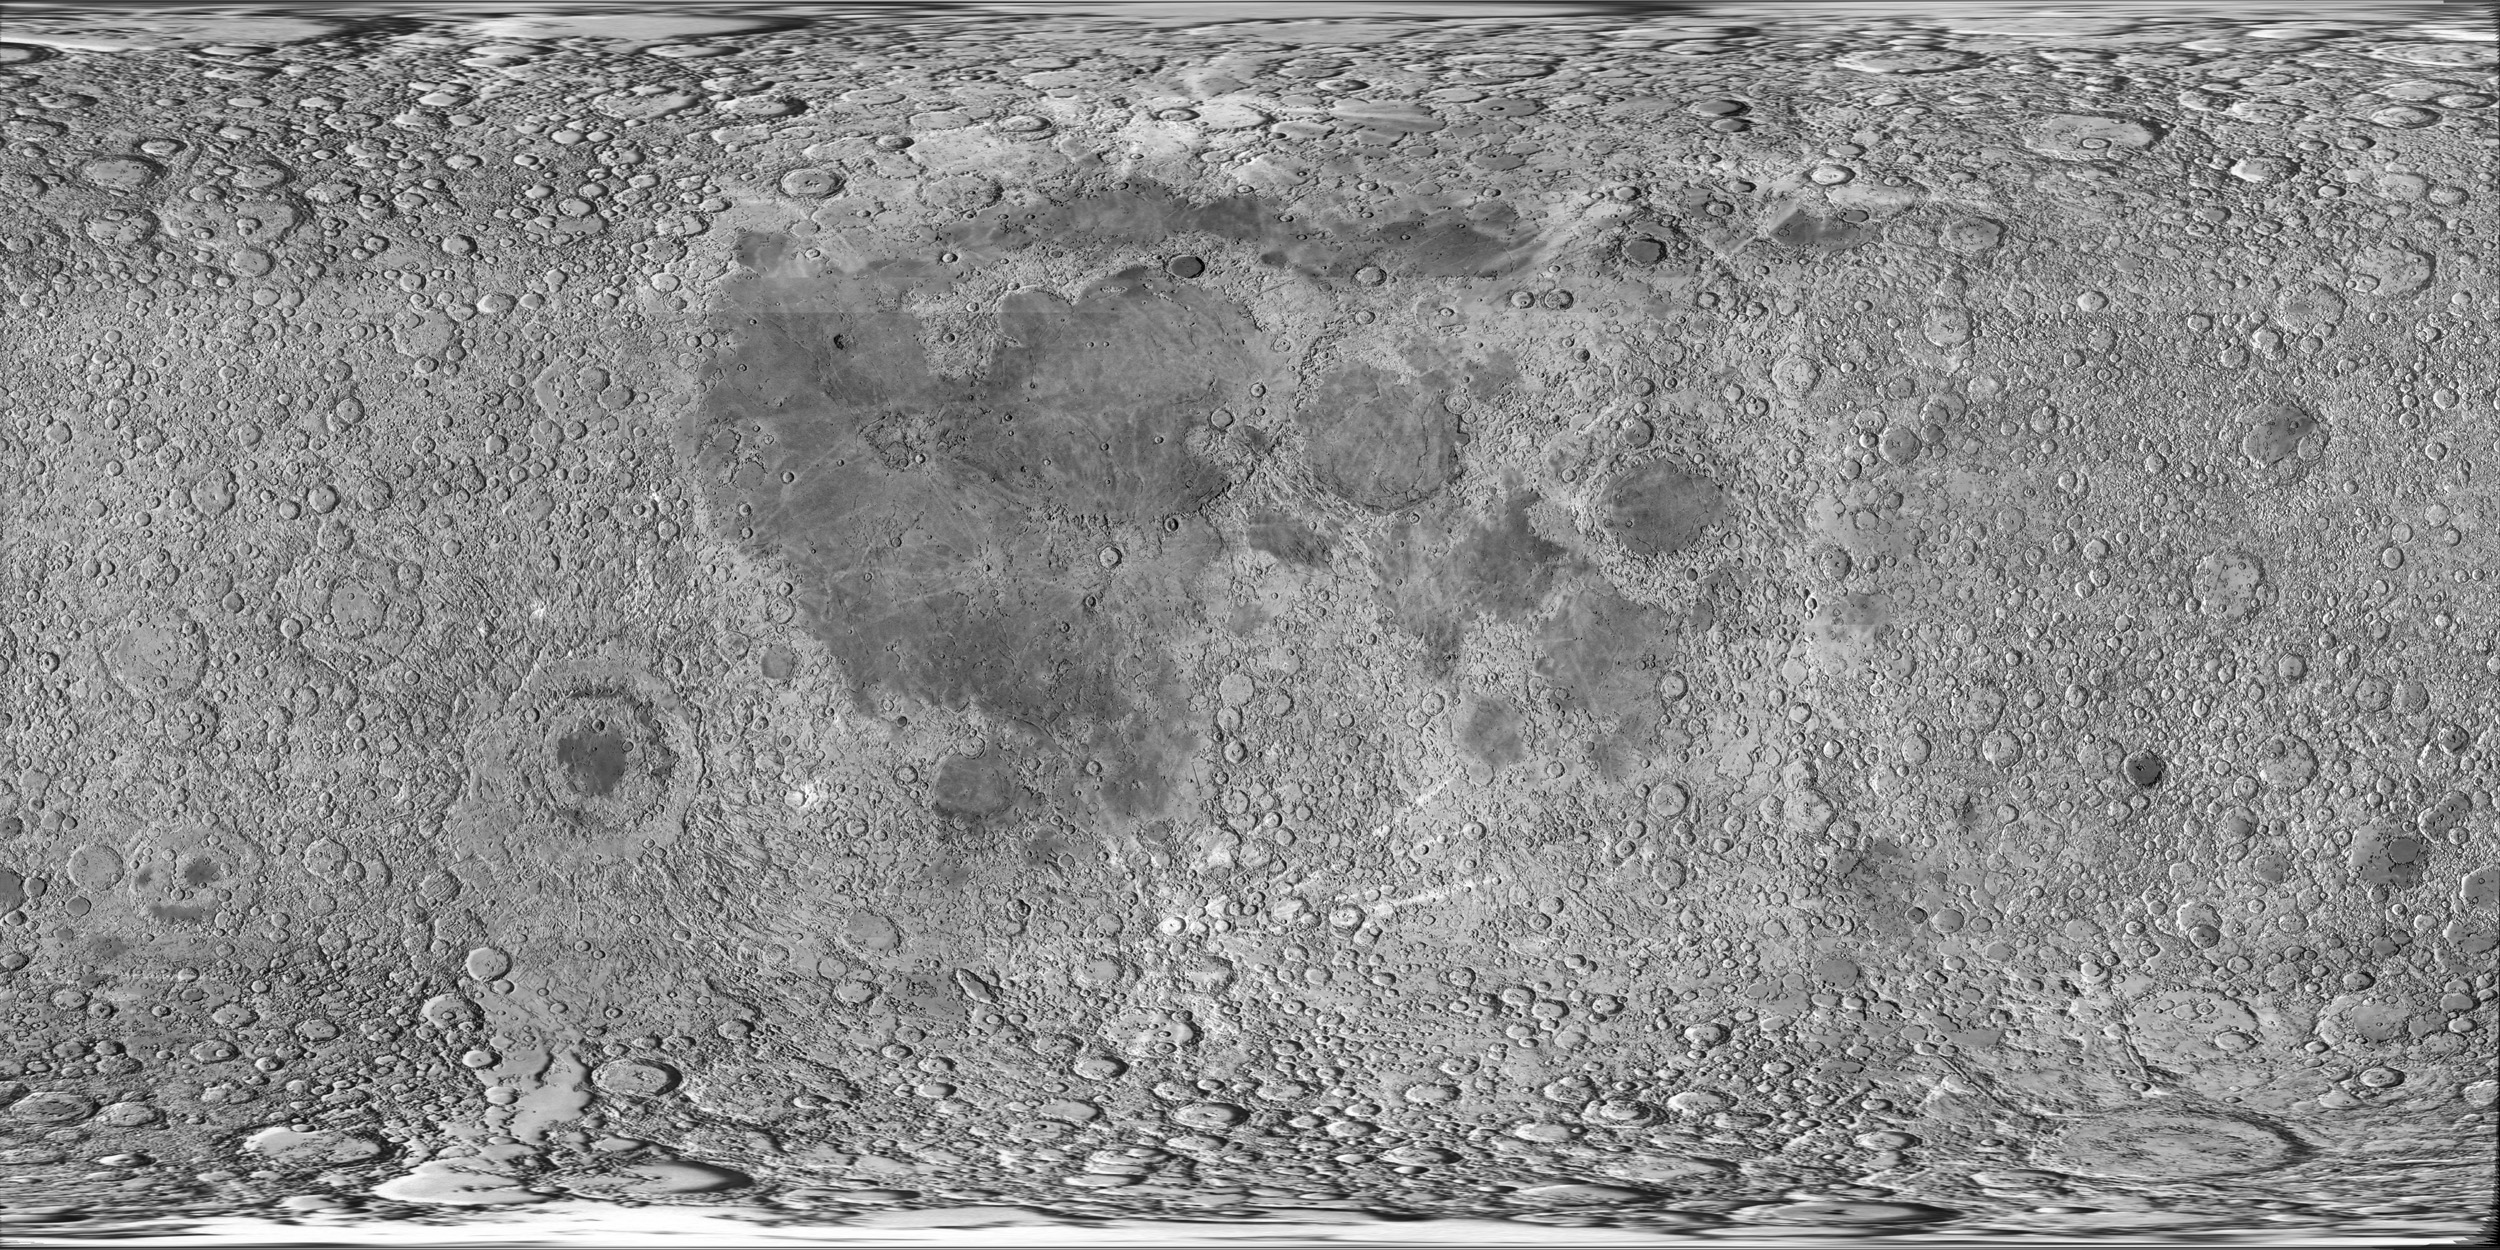
\includegraphics[width=\linewidth]{moon.jpg}
\\\\
Here is an example of it applied to a 3D sphere.
\\\\
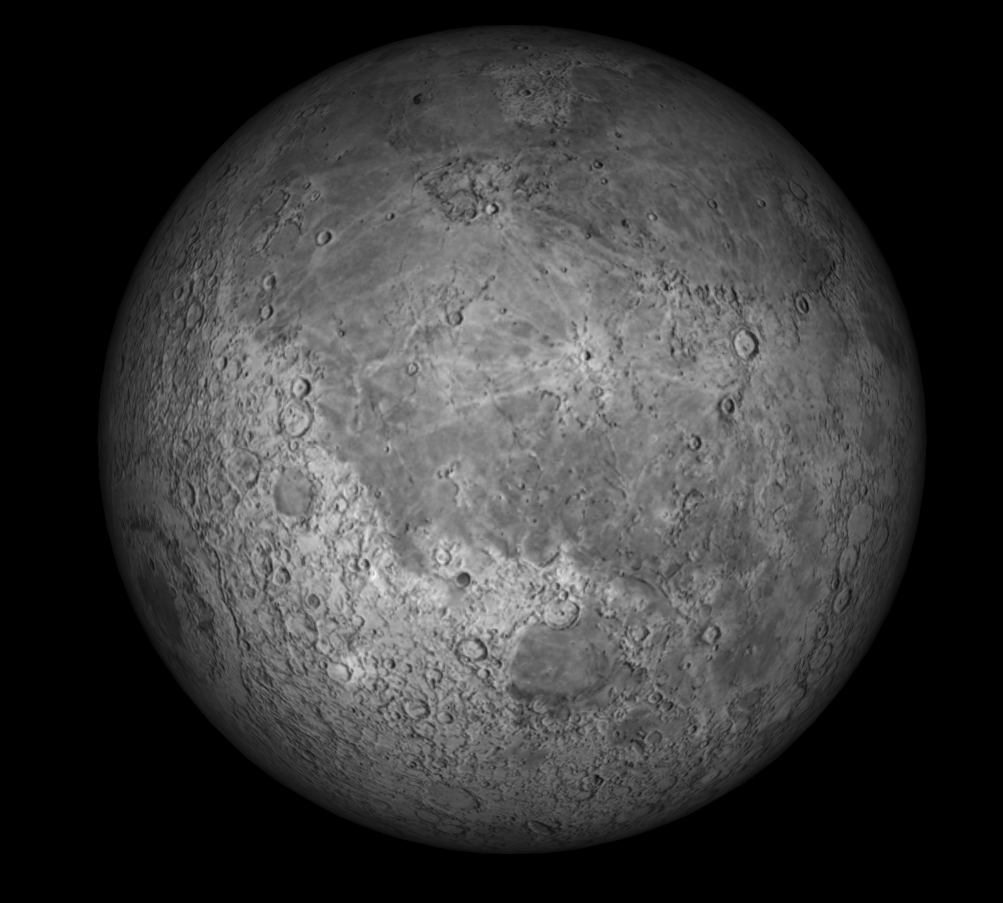
\includegraphics[width=\linewidth]{moon-sphere}
\\\\
In order to ensure that each planet was displayed when clicked on we needed to adjust our d3 code and add the "a" object with a link attribute as follows:\\
\begin{lstlisting}[frame=single]
d3.json("planet_data.json", function (data) {
  canvas.selectAll("rect")
  .data(data)
  .enter()
  .append("a")
  .attr("xlink:href", function(d) {
  switch(d.Planet) {
  case "Mercury":
  return "http://web.engr.oregonstate.edu/~se
     dwickc/cs458/mercury.html";
  case "Venus":
  return "http://web.engr.oregonstate.edu/~se
     dwickc/cs458/venus.html";
  case "Earth":
  
  ...
  
  case "Neptune":
  return "http://web.engr.oregonstate.edu/~se
      dwickc/cs458/neptune.html";
  default:
  return "http://web.engr.oregonstate.edu/~se
      dwickc/cs458/planet.html";
  break;
  }
})
\end{lstlisting}
This adds links to each object depicted in our visualization allowing the user to click on them.
The result is that each link would take the user to a 3D model of each object and allow them to interact with it.
\\\\
While we were working to add rotatable objects for users to interact with we really wanted to experiment with mapping data points to the spheres. 
What we were able to implement was a model of the Earth that allowed users to hover over certain regions and be provided with the name of the region highlighted.
Here is an example:
\\\\
Unhighlighted\\
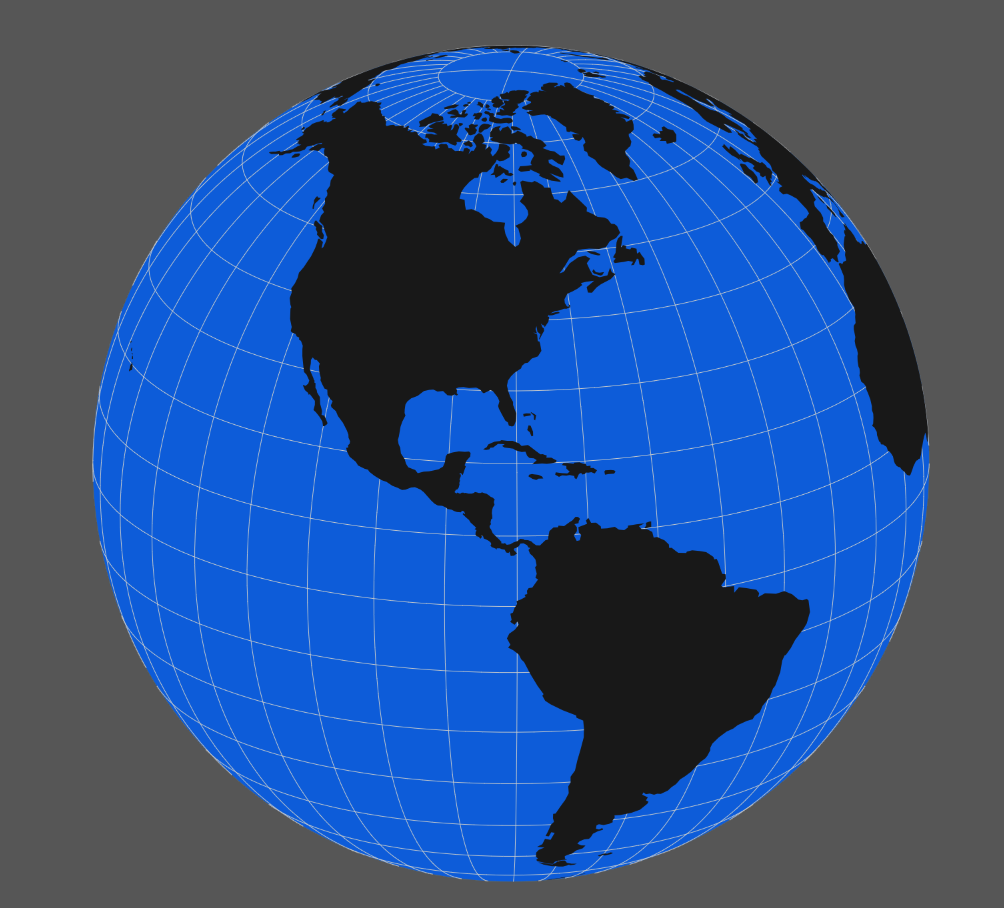
\includegraphics[width=\linewidth]{earth}
\\\\
Highlighted\\
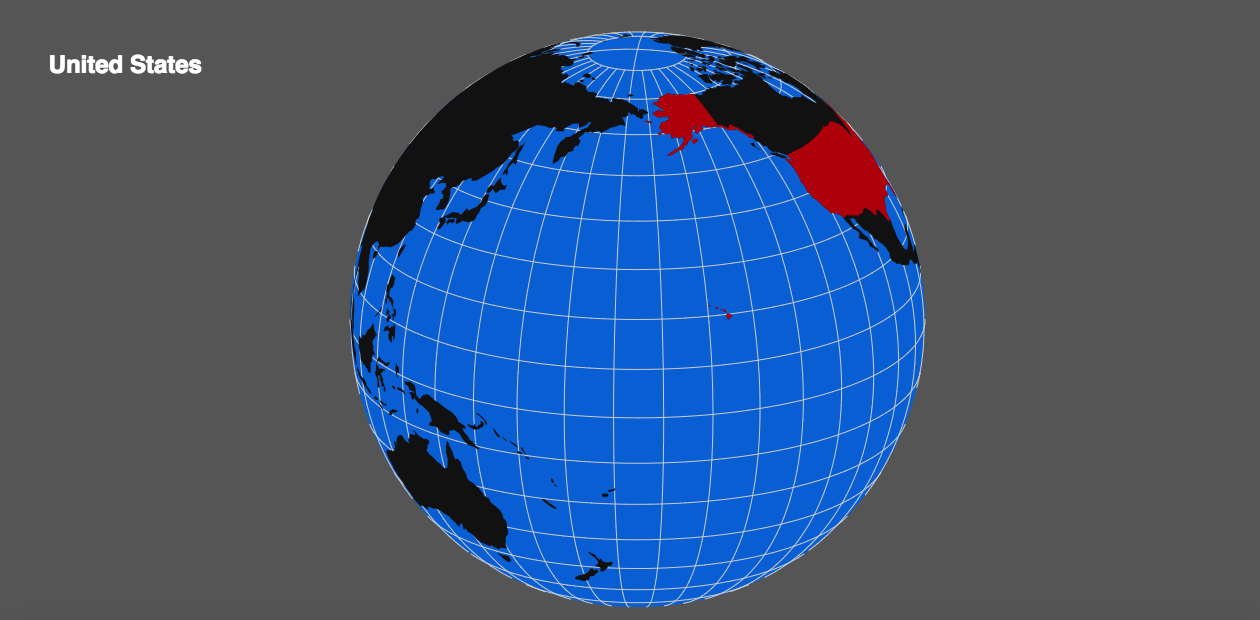
\includegraphics[width=\linewidth]{earth-selected}
\\\\
To provide users with more scientific data in our visualization we're implemented a means for users to hover over each planet and be given data relating to that planet.
The code relating to this can be found below.
\\
\begin{lstlisting}[frame=single]
<!DOCTYPE html>
<html>
<head>
<meta charset="utf-8">
<title>Interactive Solar System</title>
<script src="http://d3js.org/d3.v3.min.js">
</script>
<script src="http://labratrevenge.com/d3-
tip/javascripts/d3.tip.v0.6.3.js"></script>
<style>
body {
  background-color: #000000
}
.d3-tip {
  line-height: 1;
  font-weight: bold;
  padding: 12px;
  background: white;
  color: red;
  border-radius: 2px;
  margin-top: 45px;
}

/* Creates a small triangle 
extender for the tooltip */
.d3-tip:after {
  box-sizing: border-box;
  display: inline;
  font-size: 10px;
  font-family: sans-serif;
  width: 100%;
  line-height: 1;
  color: white;
  content: "\25BC";
  position: absolute;
  text-align: center;
}

.d3-tip.s:after {
  content: "\25B2";
  margin: 0 0 1px 0;
  top: -8px;
  left: 0;
  text-align: center;
}

</style>
</head>
<body>
<script type="text/javascript" 
src="planet_generator.js"></script>
</body>
</html>
\end{lstlisting}

\begin{lstlisting}[frame=single]
d3.json("planet_data.json", function (data) {
//Code used to place planets
	. . .
    
switch(d.Planet) {
  case "Mercury":
    tiptext = "Orbit Around the Sun: " + 
    d.Orbit + 
    "<br>Mass: " + 
    d.Mass + 
    "<br>Length of Day: " + 
    d.DayLength + 
    "<br>Length of Year: " + 
    d.YearLength + 
    "<br>Atmospheric Constituents: " + 
    d.Atmosphere + 
    "<br>Click planet to see " + 
    d.Planet + " in motion!";
  break;
  
//More switch statements like the previous one.
	. . .
    
  default:
  	tiptext=
    "http://web.engr.oregonstate.edu/
    ~kabirt/cs458/cs458_WebGL/planet.html";
  	break;
  }
  tip.html(tiptext);
  tip.show();
 })
  .on("mouseout", tip.hide);
\end{lstlisting}
%%%%%%%%%%%%%%%%%%%%%%%%%%%%%%%%%%%%%%%%%%%%%%%%%%%%%%%%%%%%%%%%%%%%
\subsection{Data}
This section covers the method we used for storing and organizing data to be used by our visualization as well as our data resource. 
%%%%%%%%%%%%%%%%%%%%%%%%%%%%%%%%%%%%%%%%%%%%%%%%%%%%%%%%%%%%%%%%%%%%
\subsubsection{Data Source}

The data we are using for this visualization comes from a compiled table of data provided by NASA.\\

\noindent The data file is included and is labeled "Solar-System-Database-by-Teoalida - Solar System.csv".\\
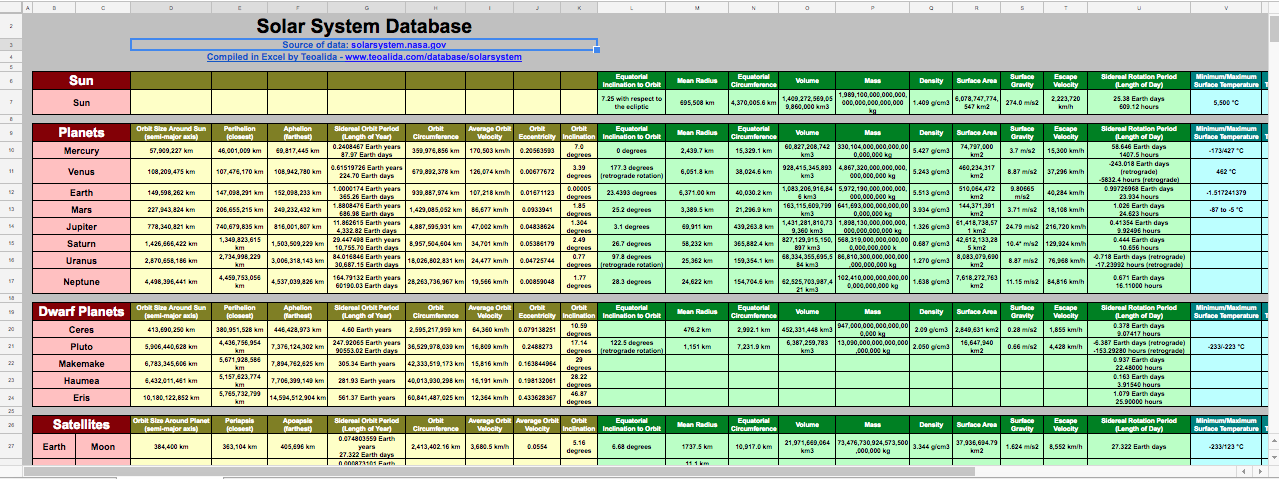
\includegraphics[width=\linewidth]{solar_data}
The table contains properties such as orbit distance from the Sun, escape velocity, surface gravity, size dimensions, and even atmospheric makeup.
%%%%%%%%%%%%%%%%%%%%%%%%%%%%%%%%%%%%%%%%%%%%%%%%%%%%%%%%%%%%%%%%%%%%
\subsubsection{Data Organization}

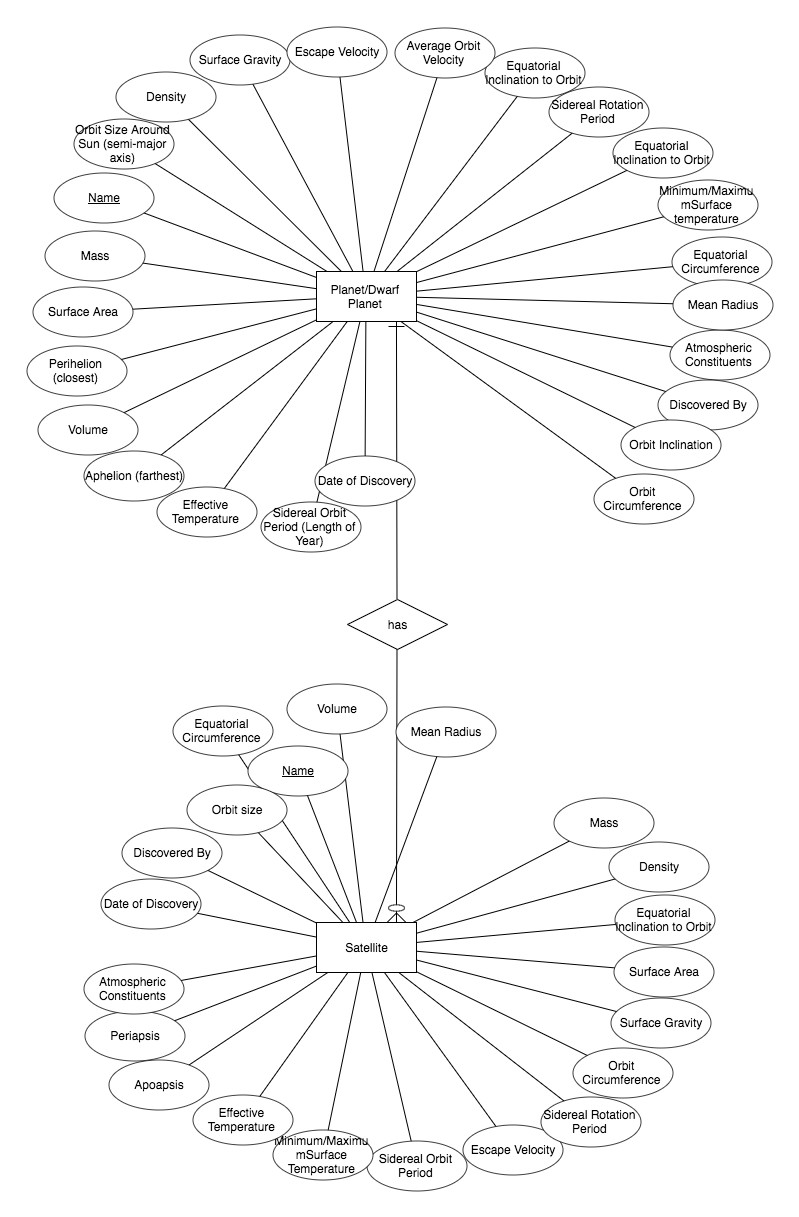
\includegraphics[width=\linewidth]{planet_sat_ERD}

\subsection{Relational Database}
We've decided to store and access our data in the form of JSON files. The files are stored in JSON files labeled "planet\_data\_edited.json" and "satellite\_data.json". The files "planet\_data\_edited.json" contain the same properties for each celestial body, but the values differ. While the "satellite\_data.json" file contains information on the planets' moons in our solar system, the "planet\_data\_edited.json"  file contains data on the eight non-dwarf planets currently in our system. All JSON objects contain the same properties with the exception of the "satellite\_data.json" file which also contains a property for the planet with which the satellite is associated with. We were able to parse through these JSON files to retreieve information about each individual celestial body. That being said, there was a lot of data in those JSON files that wasn't necessarily pertinent or interesting, so instead of displaying all of the information, we chose to implement a pop-up with some of the more relevant facts. These pop-ups are displayed when the user hovers over each individual planet. They display the respective orbit size, mass, length of day, length of year, and atmospheric constituents of each planet and also prompt the user to click on the body to see the 3D model of the planet in motion. 

\begin{lstlisting}[frame=single, basicstyle=\tiny]
{
"Planet": "Mercury",
"Orbit Size Around Sun 
(semi-major axis)": "57,909,227 km",
"Perihelion (closest)": "46,001,009 km",
"Aphelion (farthest)": "69,817,445 km",
"Sidereal Orbit Period 
(Length of Year)": "0.2408467 Earth years\n87.97 Earth days",
"Orbit_Circumference": 359976856,
"Average Orbit Velocity": "170,503 km/h",
"Orbit Eccentricity": 0.20563593,
"Orbit Inclination": "7.0 degrees",
"Equatorial Inclination to Orbit": "0 degrees",
"Mean_Radius": 2439.7,
"Equatorial Circumference": "15,329.1 km",
"Volume": "60,827,208,742 km3",
"Mass": "330,104,000,000,000,000,000,000 kg",
"Density": "5.427 g/cm3",
"Surface Area": "74,797,000 km2",
"Surface Gravity": "3.7 m/s2",
"Escape Velocity": "15,300 km/h",
"Sidereal Rotation Period (Length of Day)": "58.646 Earth days\n1407.5 hours",
"Minimum/Maximum Surface Temperature": "-173/427 °C",
"Effective Temperature": "",
"Atmospheric Constituents": "?",
"Date of Discovery": "Unknown",
"Discovered By": "Known by the Ancients",
"Color": "gray",
},
{
"Planet": "Venus",
"Orbit Size Around Sun (semi-major axis)": "108,209,475 km",
"Perihelion (closest)": "107,476,170 km",
"Aphelion (farthest)": "108,942,780 km",
"Sidereal Orbit Period (Length of Year)": 
"0.61519726 Earth years\n224.70 Earth days",
"Orbit_Circumference": 679892378,
"Average Orbit Velocity": "126,074 km/h",
"Orbit Eccentricity": 0.00677672,
"Orbit Inclination": "3.39 degrees",
"Equatorial Inclination to Orbit": "177.3 degrees (retrograde rotation)",
"Mean_Radius": 6051.8,
"Equatorial Circumference": "38,024.6 km",
"Volume": "928,415,345,893 km3",
"Mass": "4,867,320,000,000,000,000,000,000 kg",
"Density": "5.243 g/cm3",
"Surface Area": "460,234,317 km2",
"Surface Gravity": "8.87 m/s2",
"Escape Velocity": "37,296 km/h",
"Sidereal Rotation Period (Length of Day)":
"-243.018 Earth days (retrograde) -5832.4 hours (retrograde)",
"Minimum/Maximum Surface Temperature": "462 °C",
"Effective Temperature": "",
"Atmospheric Constituents": "Carbon Dioxide, Nitrogen",
"Date of Discovery": "Unknown",
"Discovered By": "Known by the Ancients",
"Color": "orange",
}

...
\end{lstlisting}

%%%%%%%%%%%%%%%%%%%%%%%%%%%%%%%%%%%%%%%%%%%%%%%%%%%%%%%%%%%%%%%%%%%%
\subsubsection{Description of the Data}
The data provided in the files including the following: the name of the celestial body, the orbit distances from the Sun (mean, closest, and farthest), the length of the year on the object (how long to make a full orbit around the Sun), the total distance covered by each orbit, the average velocity of the celestial body as it orbits the Sun, the eccentricity of the body's orbit and its inclination. Additional data provided are the equatorial inclination to orbit, the mean radius of the celestial body, the circumference of the celestial body, its volume, its mass, its density, its surface area, gravity, escape velocity, length of day (time it takes for full rotation of celestial body around its poles), the minimum and maximum surface temperature, the makeup of its atmosphere, the date it was discovered, the individual or group who discovered it and an added attribute "color" which is used primarily to facilitate visualization. 
%%%%%%%%%%%%%%%%%%%%%%%%%%%%%%%%%%%%%%%%%%%%%%%%%%%%%%%%%%%%%%%%%%%%


%%%%%%%%%%%%%%%%%%%%%%%%%%%%%%%%%%%%%%%%%%%%%%%%%%%%%%%%%%%%%%%%%%%%
\section{Results}
By implementing our code we have developed the following map for our data.\\\\
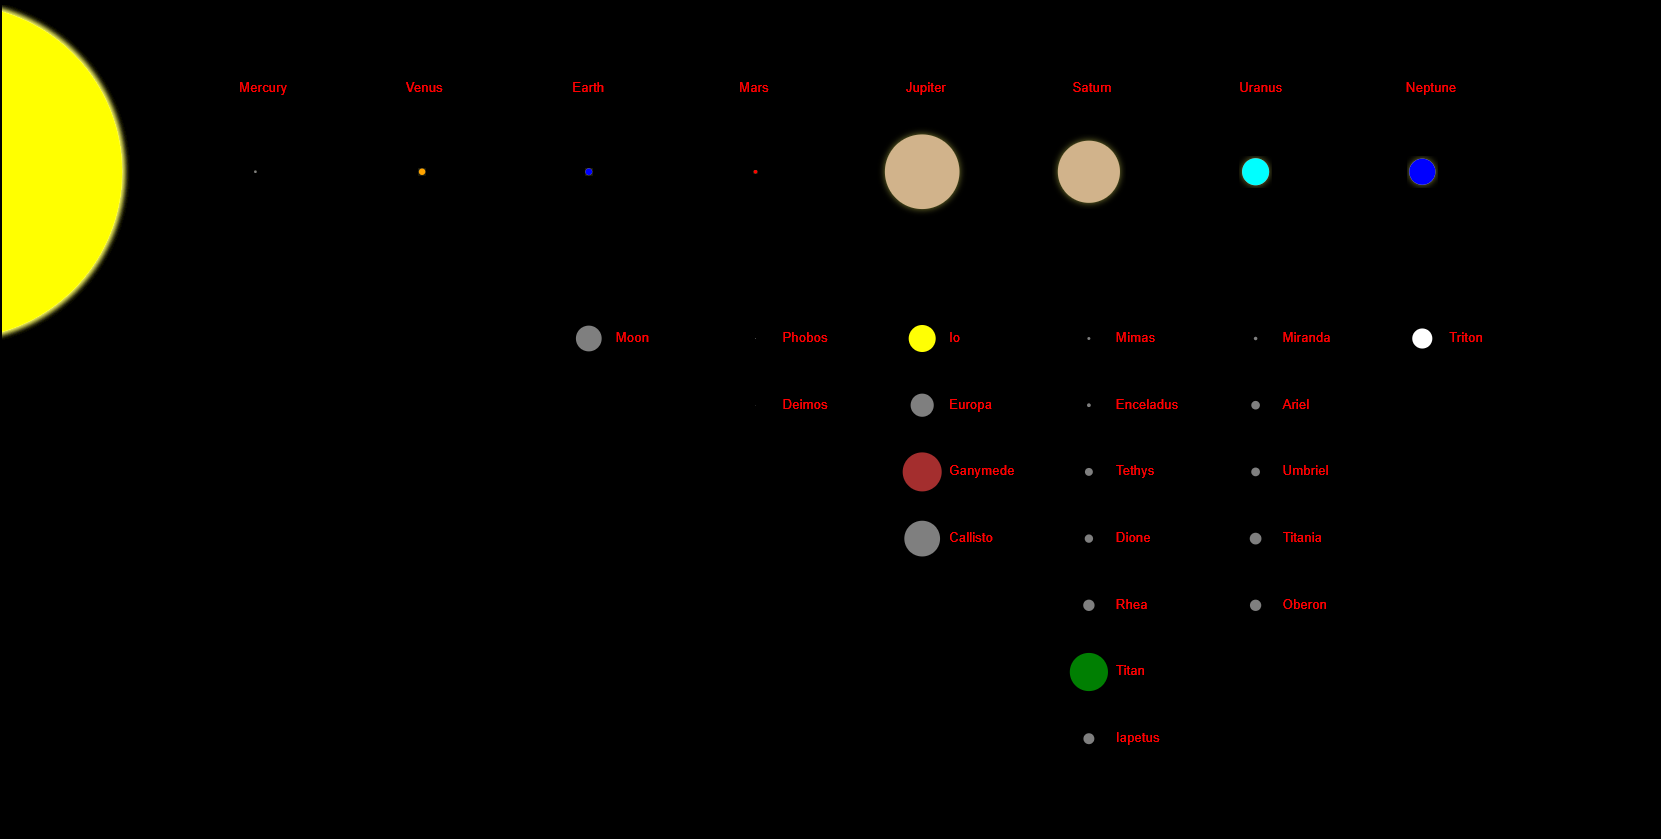
\includegraphics[width=\linewidth]{system-map}
\\\\
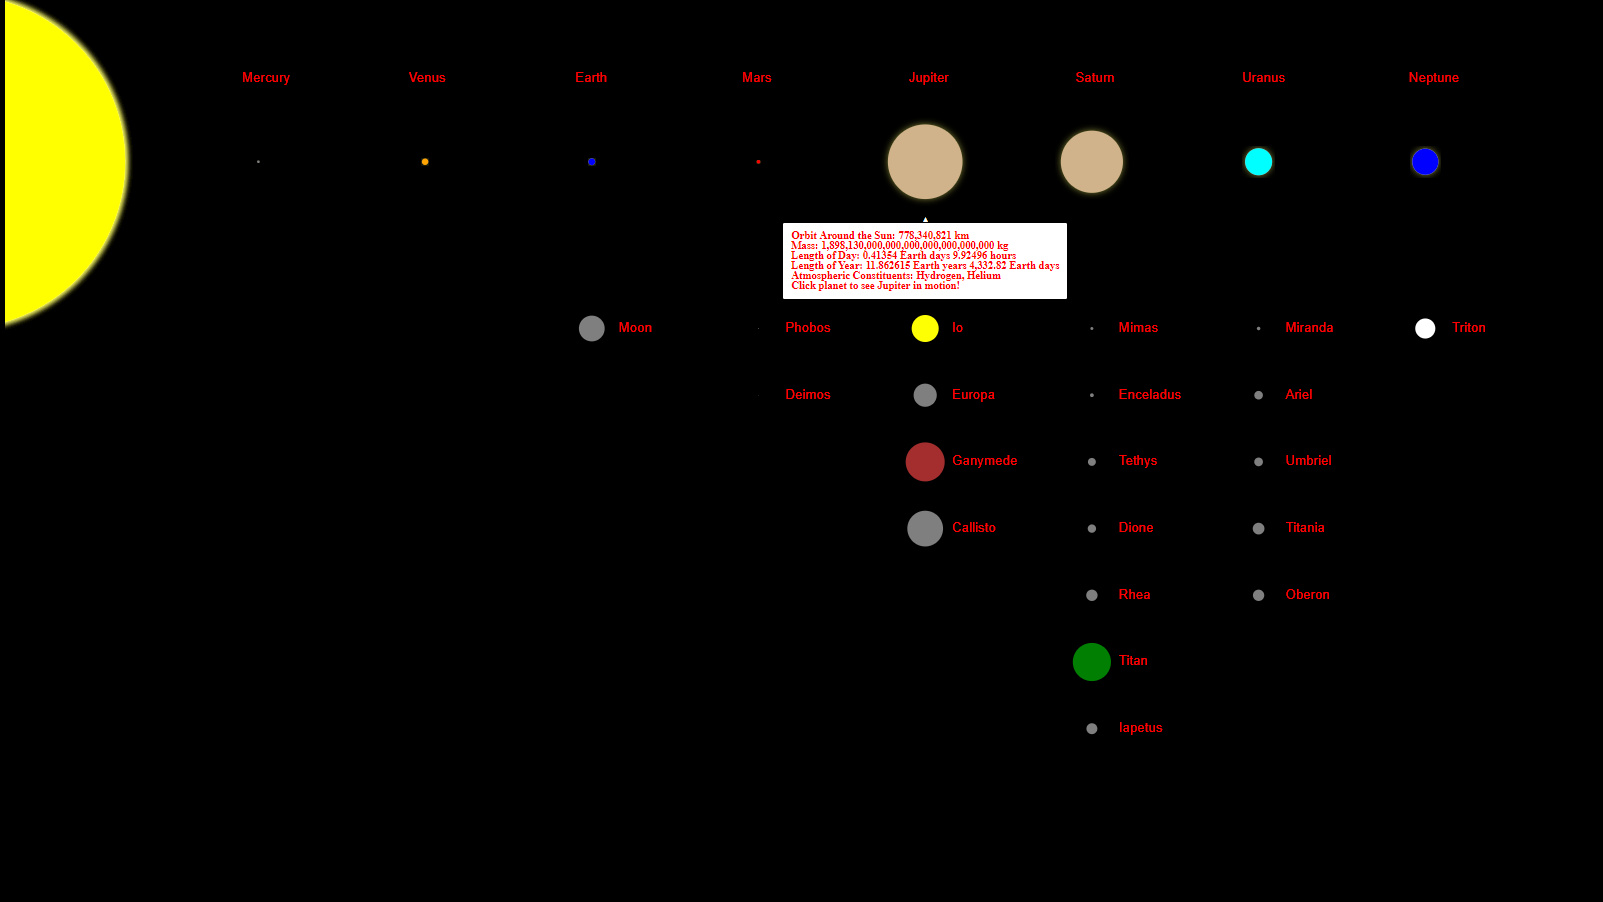
\includegraphics[width=\linewidth]{details-planet}
From the resulting depiction we can see that our visualization shows that the scale of our planet is compared to others is much different than the scaling provided by the visualization described earlier in the Related Work section.
\\\\
What this visualization shows us is that the scale of our Earth and neighboring bodies is extremely fractional compared to the size of planets such as Saturn, Neptune,  and Jupiter. We can also glean the differences in satellite sizes. Though Earth is smaller compared to other planets its satellite, the Moon, is relatively sizable compared to the satellites of the much larger planets. Another pattern to recognize is the number of satellites each planet has. It seems the further planets have many more satellites than those closer to the Sun, but the further from the Sun the number of satellites begins to decrease similar to a bell curve.
\\\\
With the addition of the textured globes for each of the planets we've implemented a means for users to get a more detailed view of the celestial bodies.
The improved models show the difference in atmosphere from each of the planets depicted. 
%%%%%%%%%%%%%%%%%%%%%%%%%%%%%%%%%%%%%%%%%%%%%%%%%%%%%%%%%%%%%%%%%%%%
\section{Conclusion}
The purpose of our visualization was to provide an easy and aesthetically pleasing way of presenting data about our solar system.  Considering the dearth of data visualizations similar to ours, we think that our interactive solar system map is needed in order to display the solar system data accurately and beautifully. This would hopefully allow users to view the data in an easy to read one-stop diagram, rather than require them to use multiple resources to view and access the same information. 
\\\\
While working on this project there have been some difficulties, but none that were insurmountable. The most difficult part when developing the visualization would have to be deciding on the layout of the visual provided to the user. We originally wanted to show both size and distance scaled, but that has proven to be difficult. When scaling distance it appears that many of our planets would appear off-screen and require scrolling to bring them into view. If we tried to scale down to account for distance then the planets and satellites would appear too small or be imperceptible to the viewer. As a compromise we have decided to visualize only size and set each object at a fixed distance. We have also scaled planets and satellites separately to account for the fact that satellites appear much smaller than their host planets.
\\\\
So far, we have been able to develop a means to scale and depict planets in our solar system according to their actual size as well as provide 3D models for users to interact with and view, create an interactive map on a 3D object, place planets in a row with their respective moons below them, show each planet’s satellites, and implement labeling as well as show details about each planet. In the future, we hope to also implement the main feature of displaying the detailed data of each celestial body when it is clicked. In order to do this in a way that does not clutter the user interface, we hope to open and display the information in a modal/pop-up when each body is clicked. This will give the user control over what they want to learn. 
\\\\
Using our technique individuals could compare magnitudes of different data values and look for patterns in their attributes. For instance, we are able to provide the user with images that show size difference on a 2D scale. If an individual wanted to look at population density of areas, they could use a similar visualization to show the population in comparison to other neighboring areas. Applying texture maps and interactive globes to display information can also be interesting tools to teach people about geography and would be great educational tools in the classroom.
%%%%%%%%%%%%%%%%%%%%%%%%%%%%%%%%%%%%%%%%%%%%%%%%%%%%%%%%%%%%%%%%%%%%
\section{Contributions}
Connor Sedwick:
\begin{itemize}
\item Set up the HTML file to be used for our web page visualization.
\item Found planet data.
\item Created JSON files.
\item Wrote d3 code for planet generation.
\item Implemented WebGL 3D modeling and textures
\item Wrote code for labeling.
\item Wrote parts of Introduction, Related Work, Method, Data, and Results sections.
\end{itemize}

\noindent Tasnia Kabir:
\begin{itemize}
\item Implemented background and coloring for website.
\item Implemented planet coloring.
\item Implemented Pop-up with information about planets.
\item Wrote parts of Introduction, Method, Data, and Conclusion sections.
\end{itemize}
%\bibliographystyle{abbrv}
%\bibliographystyle{abbrv-doi}
%\bibliographystyle{abbrv-doi-narrow}
%\bibliographystyle{abbrv-doi-hyperref}
%\bibliographystyle{abbrv-doi-hyperref-narrow}
%\bibliography{template}
\end{document}

